\documentclass[11pt,a4paper]{article}
\usepackage[T1]{fontenc}\usepackage[utf8]{inputenc}
\usepackage{amsmath,amsthm}\usepackage{newpxtext,newpxmath}
\usepackage[defaultsans]{lato}\usepackage{inconsolata}
\usepackage[a4paper,top=24mm,bottom=23mm,left=24mm,right=24mm,headsep=9mm]{geometry}
\usepackage{microtype,mathtools,graphicx,booktabs,longtable,tabularx,array,multirow}
\usepackage[table]{xcolor}\usepackage{tikz}
\usetikzlibrary{arrows.meta,positioning,calc,shapes.geometric}
\usepackage[most]{tcolorbox}\usepackage{fancyhdr,titlesec,caption,float,needspace,listings,url}
\usepackage[unicode,pdfencoding=auto]{hyperref}
\definecolor{navy}{HTML}{102E3A}\definecolor{teal}{HTML}{107B80}
\definecolor{slate}{HTML}{586B73}\definecolor{pale}{HTML}{F0F5F5}
\definecolor{gold}{HTML}{B59555}\definecolor{rulegray}{HTML}{D3DFE1}
\definecolor{pr}{HTML}{C43B3B}\definecolor{po}{HTML}{D87518}\definecolor{py}{HTML}{D3AD24}
\definecolor{pg}{HTML}{26835D}\definecolor{pb}{HTML}{2875B6}\definecolor{pi}{HTML}{514FA3}\definecolor{pv}{HTML}{914DA8}
\hypersetup{colorlinks=true,linkcolor=navy,urlcolor=teal,pdfauthor={Tom Klootwijk},
 pdftitle={UU ID Prism - Unified Field Theory V2.1.1},pdfsubject={Rainbow facets, holder-scoped legacy-data migration and personal data passport},
 pdfkeywords={UU ID, Prism, rainbow, sensory facets, provenance, personal data passport, Tom Klootwijk}}
\AtBeginDocument{\fontsize{10.5}{13}\selectfont\setlength{\abovedisplayskip}{7pt plus 2pt minus 2pt}\setlength{\belowdisplayskip}{7pt plus 2pt minus 2pt}}
\setlength{\parindent}{0pt}\setlength{\parskip}{5pt}\setlength{\emergencystretch}{2em}\setlength{\headheight}{15pt}
\setlength{\tabcolsep}{5pt}\renewcommand{\arraystretch}{1.15}
\pagestyle{fancy}\fancyhf{}\fancyhead[L]{\sffamily\scriptsize\color{slate}TOM KLOOTWIJK}
\fancyhead[R]{\sffamily\scriptsize\color{slate}V2.1.1 / UU ID PRISM}
\fancyfoot[L]{\sffamily\scriptsize\color{slate}SUB-ADDENDUM TO V2.1.0}\fancyfoot[R]{\sffamily\small\thepage}
\renewcommand{\headrulewidth}{.3pt}
\titleformat{\section}{\sffamily\LARGE\bfseries\color{navy}}{\thesection}{.6em}{}
\titleformat{\subsection}{\sffamily\Large\bfseries\color{navy}}{\thesubsection}{.6em}{}
\titleformat{\subsubsection}{\sffamily\normalsize\bfseries\color{teal}}{}{0em}{}
\titlespacing*{\section}{0pt}{0pt}{12pt}\titlespacing*{\subsection}{0pt}{0pt}{12pt}\titlespacing*{\subsubsection}{0pt}{10pt}{4pt}
\captionsetup{font=small,labelfont={bf,sf},labelsep=period,skip=7pt}
\newcommand{\newpagehead}[1]{\clearpage\subsection{#1}}
\newcommand{\source}[1]{{\sffamily\small\color{slate}[#1]}}
\newcommand{\uu}{\operatorname{UU\,ID}}\newcommand{\ind}{\mathbf{1}}\newcommand{\clip}{\operatorname{clip}}
\newcommand{\band}[2]{\colorbox{#1}{\strut\makebox[11pt]{\color{white}\sffamily\bfseries #2}}}
\newtcolorbox{formal}[1]{enhanced,breakable,colback=pale,colframe=teal,boxrule=.55pt,sharp corners,left=10pt,right=10pt,top=8pt,bottom=8pt,coltitle=white,colbacktitle=teal,fonttitle=\sffamily\bfseries,title={#1},before skip=9pt,after skip=9pt}
\newtcolorbox{note}[1]{enhanced,breakable,colback=white,colframe=rulegray,boxrule=.6pt,borderline west={2pt}{0pt}{gold},sharp corners,left=10pt,right=10pt,top=8pt,bottom=8pt,fonttitle=\sffamily\bfseries,coltitle=navy,colbacktitle=pale,title={#1},before skip=9pt,after skip=9pt}
\lstset{basicstyle=\ttfamily\small,breaklines=true,columns=fullflexible,keepspaces=true,frame=single,rulecolor=\color{rulegray},backgroundcolor=\color{pale},showstringspaces=false,aboveskip=8pt,belowskip=8pt}
\renewcommand{\thesection}{I}\numberwithin{equation}{section}
\begin{document}\setcounter{page}{46}\setcounter{section}{0}\section{UU ID Prism}
\subsection{From legacy fragments to a personal passport}
\textbf{Release 2.1.1.} Sub-addendum to the supplied \emph{Unified Field Theory V2.1}, treated as semantic parent \texttt{2.1.0}. Author: \textbf{Tom Klootwijk}, NL200678942, 10-07-1990. The author record remains documentary attribution; the executable examples use a separate synthetic holder.

The \emph{UU ID Prism} is a labelled projection of an individual's authorized data records into seven rainbow bands. Each band identifies a domain; each facet retains its record references, provenance, permission state and observation time. The aim is a finite, practical migration from scattered legacy exports into an inspectable \emph{personal data passport}, rather than another continuously ranked feed.

\begin{formal}{Definition P0: the Prism is a view, not a new identity classifier}
For holder $s$, admitted records $A_s(t)$ and versioned facet registry $\mathcal R$, define
\[
\operatorname{Prism}_{\mathcal R}(s,t)
  =\big\langle (f,\kappa(f),V_{s,f}(t),\Lambda_{s,f}(t))\big\rangle_{f\in\mathcal F}.
\]
$f$ names a facet, $\kappa(f)$ its display band, $V_{s,f}$ its explicitly defined summary and $\Lambda_{s,f}$ its references and lineage. The source records remain separate from their visualization.
\end{formal}

\begin{figure}[H]\centering
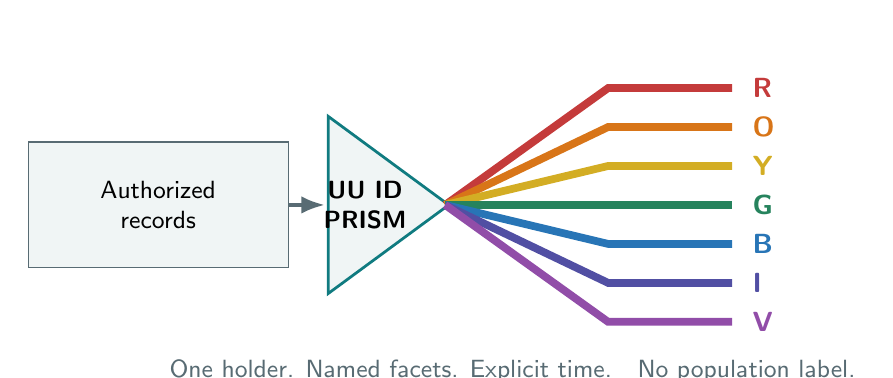
\begin{tikzpicture}[>=Latex,scale=.9,every node/.style={font=\sffamily\small}]
\node[draw=slate,fill=pale,align=center,minimum width=33mm,minimum height=16mm] (in) at (0,0) {Authorized\\records};
\draw[teal,fill=pale,line width=1pt] (2.4,-1.25)--(2.4,1.25)--(4.1,0)--cycle;
\node[align=center,font=\sffamily\bfseries\small] at (2.92,0) {UU ID\\PRISM};
\draw[->,slate,line width=1.2pt] (in.east)--(2.35,0);
\foreach \y/\col/\lab in {1.65/pr/R,1.10/po/O,.55/py/Y,0/pg/G,-.55/pb/B,-1.10/pi/I,-1.65/pv/V}{
\draw[\col,line width=2.8pt] (4.05,0)--(6.35,\y)--(8.1,\y);
\node[anchor=west,text=\col,font=\sffamily\bfseries] at (8.25,\y) {\lab};}
\node[align=center,text=slate] at (5,-2.35) {One holder. Named facets. Explicit time.\quad No population label.};
\end{tikzpicture}
\caption{The prism is a routing and presentation metaphor. Color indexes the declared data facet; no optical or intelligence-collection device is implied.}
\end{figure}

The attached dialogue supplies the prism, rainbow and total-aggregation scenario. This addendum preserves that conceptual origin and identifies its unsupported extrapolations explicitly. The implemented branch is \textbf{holder-governed inventory and metadata migration}; the NSA mass-harvesting and \emph{divide et impera} discussion is retained as a scenario and governance concern, not as a deployed collection design. \source{S5; I.2; I.15--I.16}

\newpagehead{Source meanings and the PRISM distinction}
\subsubsection{What the supplied dialogue contributes}
The Markdown dialogue moves from \emph{Shunyata}, signal/noise and wave propagation to prism dispersion, a replicated rainbow symbol, active-bit extraction, packed words, state-field geometry, a hypothetical passport and total data aggregation. Its later passages assert that parity, latches and gaze would expose concealed traits or stabilize universal behavioral groups. These are statements in the supplied conversation; they are not new measurements or additional proofs in the V2 corpus. \source{S5, thematic sequence}

\begin{center}\small\begin{tabularx}{\textwidth}{@{}p{.23\textwidth}X@{}}\toprule
\textbf{Term} & \textbf{Meaning used in this addendum}\\\midrule
UU ID & The corpus's minimum of absolute threshold deviations, with labelled components retained.\\[5pt]
Prism & A new typed partition and display of authorized records across named facets.\\[5pt]
Rainbow spectrum & A categorical visual vocabulary, not a measurement of a person's electromagnetic signature.\\[5pt]
NSA PRISM & A historically documented intelligence-collection name, distinguished from the new Prism software.\\[5pt]
Digital passport & A holder-scoped, versioned personal-data manifest and view. It is not an issued border-crossing credential.\\[5pt]
``All data'' & All records within an explicit inventory, authorization and import scope at a stated time.\\\bottomrule
\end{tabularx}\end{center}

\subsubsection{A separately checked historical point}
The 2023 Privacy and Civil Liberties Oversight Board report describes downstream collection, previously called PRISM, as collection from electronic communications service providers using identified selectors. It distinguishes that process from upstream acquisition of communications in transit over the telecommunications backbone. This is a historical source distinction, not a claim about the present operational reach of any agency. \source{E1, printed pp. 3--4}

Neither that distinction nor the supplied corpus establishes that every individual's sensory experience, iris motion or private preference has been captured. The new software has no NSA connection, interception interface, camera or microphone access. No person-level data were obtained for this edition.

\subsubsection{Symbol, spiritual interpretation and evidence}
A rainbow palette can be selected without asserting that the Pride flag is a collection mechanism, that displaying it identifies someone's sexuality, or that a social movement is a hidden data structure. The supplied files provide no acquisition evidence for those assertions. The Shunyata and audio-company discussion remains conceptual background; it is not imported as a technical specification or a verified biographical chain.

The Christian monotheistic interpretation in Appendix H is retained unchanged. Its source--boundary roles do not become metadata labels assigned to people, moral scores, or criteria for grouping religious communities. \source{B, Appendix H}

\newpagehead{The seven-band spectral vocabulary}
The profile \texttt{UU-PRISM-35-1} defines seven bands, with five named facets per band. These assignments are \textbf{new design choices} in version 2.1.1. The earlier sources do not supply a sensory color taxonomy. Each band is stable within this profile and has both a letter and a plain-language name.

\begin{center}\begin{tabularx}{\textwidth}{@{}p{.07\textwidth}p{.16\textwidth}Xp{.18\textwidth}@{}}\toprule
\textbf{Code} & \textbf{Color} & \textbf{Domain} & \textbf{Facet IDs}\\\midrule
\band{pr}{R} & Red & Vision and visual context & F01--F05\\[10pt]
\band{po}{O} & Orange & Sound and language & F06--F10\\[10pt]
\band{py}{Y} & Yellow & Touch, motion and orientation & F11--F15\\[10pt]
\band{pg}{G} & Green & Body, chemical senses and environment & F16--F20\\[10pt]
\band{pb}{B} & Blue & Place, activity and time & F21--F25\\[10pt]
\band{pi}{I} & Indigo & Expression, learning and relationships & F26--F30\\[10pt]
\band{pv}{V} & Violet & Identity, rights and provenance & F31--F35\\\bottomrule
\end{tabularx}\end{center}

\subsubsection{Facet, modality and value are different fields}
A \emph{facet} identifies what a record concerns. A \emph{modality} identifies how its source says it was acquired: imported file, direct measurement or voluntary self-report. A \emph{value} requires its own units, calibration and interpretation. A text journal about taste is not a chemical sensor measurement; a gaze coordinate is not an iris identity template; a sleep estimate is not interchangeable with an original physiological signal.

A complete measurement extension therefore declares a modality record
\[
 m=(\mathrm{source},\mathrm{quantity},\mathrm{unit},\mathrm{calibration},
       \mathrm{resolution},\mathrm{uncertainty},\mathrm{transform\_version}).
\]
The shipped prototype does not fabricate these fields. It indexes payload references and their metadata; the original values remain in the holder's source files.

\begin{note}{Literal labeling without a color-only interface}
The same facet ID, domain name and status text accompany every band. Hue never means good/bad, truthful/deceptive, religious affiliation, sexuality or risk. W3C's Use of Color criterion requires an additional visual means when color conveys meaning; this design therefore retains readable labels and counts. \source{E4}
\end{note}

The RGB color values are presentation codes in \texttt{spec/facets.json}. No wavelength in nanometers is assigned to a personal characteristic. New facets require an explicit profile revision; they are not silently inserted into a pre-existing person's band.

\newpagehead{Facet catalogue: sensory and environmental records}
\source{V2.1.1 construction; machine-readable catalogue: spec/facets.json and spec/facets.csv}
\begin{center}\small\begin{tabularx}{\textwidth}{@{}p{.09\textwidth}p{.30\textwidth}X@{}}\toprule
\textbf{Facet} & \textbf{Label} & \textbf{Admitted record meaning}\\\midrule
F01 & Still imagery & Holder-selected photo references and capture metadata.\\[5pt]
F02 & Video and visual sequences & Video references, sequence identifiers and recorded context.\\[5pt]
F03 & Gaze and fixation & Authorized gaze coordinates with a calibration record; no trait inference.\\[5pt]
F04 & Screen and visual context & Holder-selected screen or window-event exports.\\[5pt]
F05 & Visual accessibility & Voluntarily entered visual-access requirements.\\\midrule
F06 & Audio recordings & Holder-owned or approved audio references.\\[5pt]
F07 & Speech and transcripts & Approved transcripts or speech records; participant permission remains explicit.\\[5pt]
F08 & Acoustic observations & Sound quantities with their stated units and source calibration.\\[5pt]
F09 & Listening history & Holder-exported playback and listening events.\\[5pt]
F10 & Communication records & Selected message metadata with third-party information minimized.\\\midrule
F11 & Touch and pressure & Contact, pressure or surface-temperature observations.\\[5pt]
F12 & Haptic interactions & Device-reported haptic input/output events.\\[5pt]
F13 & Movement and acceleration & Authorized motion and inertial-sensor records.\\[5pt]
F14 & Posture and proprioception & Recorded posture or the holder's report of body position.\\[5pt]
F15 & Balance and orientation & Authorized orientation or balance observations.\\\midrule
F16 & Physiological observations & Holder-approved references to physiological records.\\[5pt]
F17 & Sleep and rest & Holder-exported sleep or rest records; source method retained.\\[5pt]
F18 & Taste and food experience & Voluntary sensory journal entries, not inferred preferences.\\[5pt]
F19 & Smell and air observations & Separate self-reports of smell and labelled air-sensor observations.\\[5pt]
F20 & Environmental context & Ambient light, temperature or other declared environmental records.\\\bottomrule
\end{tabularx}\end{center}

\textbf{Default state: disabled and private.} Registry inclusion does not enable a sensor or imply that a measurement exists. A selected local import is the only acquisition mechanism implemented here. Gaze, communications, body-related data and other restricted facets remain holder-scoped.

\newpagehead{Facet catalogue: lived context and documentary identity}
\begin{center}\small\begin{tabularx}{\textwidth}{@{}p{.09\textwidth}p{.30\textwidth}X@{}}\toprule
\textbf{Facet} & \textbf{Label} & \textbf{Admitted record meaning}\\\midrule
F21 & Location & Authorized place records; a coarse view is the deployment default.\\[5pt]
F22 & Journeys and transport & Selected travel, journey or transport exports.\\[5pt]
F23 & Calendar and routine & Selected appointments and holder-defined routines.\\[5pt]
F24 & Application use and screen time & Holder-exported session durations or activity records.\\[5pt]
F25 & Transactions and activity & Selected receipts or activity records; no inferred wealth ranking.\\\midrule
F26 & Authored work & Documents, creations and project references selected by the holder.\\[5pt]
F27 & Learning and skills & Courses, projects and holder-maintained skills records.\\[5pt]
F28 & Relationships and permissions & Selected contact permissions, not a population relationship graph.\\[5pt]
F29 & Experience and self-report & Voluntary journal records; no hidden mental-state classification.\\[5pt]
F30 & Voluntary identity declarations & Optional self-description, belief or sexuality statements supplied by the holder.\\\midrule
F31 & Holder identity records & Private holder anchor and approved identity-document references.\\[5pt]
F32 & Issuer credentials & References carrying issuer, status and verification information.\\[5pt]
F33 & Consent and purpose & Permission receipts, declared scope and expiry.\\[5pt]
F34 & Correction and withdrawal & Correction, revocation and retention decisions.\\[5pt]
F35 & Provenance and lineage & Source manifests, transform versions and integrity references.\\\bottomrule
\end{tabularx}\end{center}

\subsubsection{Open-world coverage}
The 35 facets are an extensible administrative and sensory registry, not a proof that human experience has exactly 35 dimensions. A source outside the registry is \emph{unmapped}, not squeezed into an unrelated label. A planned but unimported source remains \emph{missing}; a source that was never planned remains \emph{not planned}. Neither state asserts that the person lacks that experience or attribute.

\subsubsection{Private declarations are not computed from other bands}
F30 is optional and accepts self-reported or synthetic declarations in this prototype. It is not populated from gaze, media choices, location, friends, body measurements, symbols or the author's spiritual interpretation. These cross-domain inferences are absent from the admitted operator set.

The source's proposed ``spectra of all facets of human life'' is therefore incorporated as a \emph{labelled, expandable record space}. The individual remains the subject who can inspect and correct their records, rather than a class inferred from a color. \source{S5; new profile UU-PRISM-35-1}

\newpagehead{The passport state and the meaning of all}
\begin{formal}{Definition P1: personal-data passport state}
For one holder $s$, define
\[
 P_{s,n}=(u_s,\mathcal R,\mathcal M_s,O_s,L_{s,n},A_{s,n},W_{s,n},\Pi_s).
\]
$u_s$ is a private holder reference; $\mathcal R$ the versioned facet registry; $\mathcal M_s$ the selected import plan; $O_s$ the referenced object metadata; $L_{s,n}$ the ordered event record; $A_{s,n}$ the current admitted links; $W_{s,n}$ the withdrawn-link set; and $\Pi_s$ the local permission policy.
\end{formal}

The reference is an identifier, not a password, proof of citizenship or proof of a complete human identity. The corpus's \emph{UU ID} operator and the conventional \emph{UUID} identifier standard are different notions. RFC 9562 defines UUIDs as 128-bit identifiers and explicitly rejects treating their possession as an access capability. A deployment may use random opaque identifiers without changing the UU ID equations. \source{E3, Sections 4, 5.4 and 8}

\subsubsection{The totality quantifier}
Let $\mathcal M_s$ enumerate the holder's chosen legacy scope. A candidate record belongs to the operational scope only after type checks, an explicit permission declaration, a confirmed subject link and conflict resolution. At time $t$,
\[
 A_s(t)=\{r\in\mathcal M_s:\operatorname{admitted}(r)\land
           \operatorname{permitted}(r,t)\land\neg\operatorname{withdrawn}(r,t)\}.
\]
``All'' means the entirety of this finite declared scope. It does not identify all data held anywhere by third parties, prove that hidden data exists, or fill unobserved life events with guessed values. An unavailable source can be listed as unavailable without claiming access to it.

\subsubsection{One holder, many sources, no automatic identity fusion}
Different accounts, filenames and equal content hashes can refer to the same or different people. Equality of data does not decide equality of subjects. The prototype requires the same explicit holder reference and \texttt{holder\_confirmed} link declaration. It quarantines a mismatched holder; it does not search for or infer another person's records.

The author identifier NL200678942 remains in the document's attribution record. It is not used as a global join key, a sensor calibration constant or the seed for the synthetic data. The demonstration uses \texttt{holder:synthetic-001}.

\begin{note}{Finite engine state versus an expanding archive}
The $118N+27$-bit Gambit word encodes the admitted engine state defined in the parent corpus. A growing personal archive has its own storage and input-driven updates. It is not silently fitted into that fixed word. The parent numerical recurrence and the new record archive are separate coordinates. \source{B, Sections 6--9}
\end{note}

\newpagehead{UU ID applied to labelled migration horizons}
The parent definition is retained:
\[
 \delta_f(x)=|d_f(x)-T_f|,\qquad
 U_F(x)=\min_{f\in F}\delta_f(x),\qquad U_\varnothing=+\infty.
\]
The software represents an empty family by \texttt{null}, rather than an infinite JSON number. The normalized horizon remains a scalar observable; the component labels remain separate. \source{B, Section 2}

\subsubsection{A fully specified migration observable}
The executable example uses a narrow, explicit quantity: \emph{coverage of planned metadata slots}. Let $n_f(t)$ be active admitted record links for facet $f$ and $m_f$ its declared positive target. Define
\begin{align}
 c_f(t)&=\min\{1,n_f(t)/m_f\},&&m_f>0,\\
 T_f&=1,\qquad\delta_f(t)=|c_f(t)-1|,\\
 U_s(t)&=\min_{f:m_f>0}\delta_f(t).
\end{align}
The implementation uses exact rational numbers. A facet with target zero has no coverage fraction and is omitted from this minimum. Its status is \emph{not planned}. These quantities are dimensionless migration-accounting values, not sensory intensity, health, identity strength or compliance scores.

\begin{formal}{Definition P2: retain the complete spectral vector}
The passport retains
\[
 \mathcal P_s(t)=\big(U_s(t),\langle f,c_f(t),\delta_f(t),\mathrm{status}_f,
   \mathrm{time}_f,\mathrm{references}_f\rangle_{f\in\mathcal F}\big).
\]
The minimum and its attaining component IDs can be queried, but the minimum never replaces the vector or the archive.
\end{formal}

\subsubsection{A zero minimum is not complete migration}
For two planned facets with $c_1=1$ and $c_2=0$, the UU ID minimum is zero while one facet is missing. The correct whole-plan condition is
\[
 \operatorname{Complete}(s,t)=\bigwedge_{f:m_f>0}[n_f(t)\ge m_f].
\]
The empty-plan result is \emph{not planned}, represented by \texttt{null}. The demonstration deliberately records a zero UU minimum and a false whole-plan condition, exposing this distinction rather than hiding it in a composite color.

\subsubsection{Extensions to real measurements}
A future measurement adapter must specify $d_f$, its units, its normalization and its threshold before an absolute deviation is evaluated. Combining unrelated raw quantities such as pixels, degrees and milliseconds by a minimum has no declared meaning. The shipped calculation uses coverage only; no private human characteristic is inferred by choosing a threshold.

\newpagehead{Formal invariants of the Prism extension}
\subsubsection{P3. Admission, replay and duplicate invariance}
For a fixed registry, permission rule and ordered candidate sequence, the validator has a deterministic outcome: admit, correct, duplicate or quarantine. An exact retry of a previously admitted record leaves the current record view and event root unchanged; the receipt's duplicate-attempt counter increments. A correction must name the digest of the preceding record version. Withdrawal removes a link from active projection without rewriting prior events.

\emph{Argument.} Field validation, ID lookup, content equality and predecessor comparison are explicit deterministic predicates. The corresponding branch has one defined update. Induction over the candidate sequence gives one record view and event sequence. Duplicate handling does not append an event, so the stated invariant follows. This is an invariant of the specified local metadata processor, not proof that the input declarations are truthful.

\subsubsection{P4. Label preservation and non-injective summaries}
A projection that retains facet IDs and record references preserves which admitted records contributed to each band. A projection to one count, one parity bit, one minimum or a bounded RGB token is generally non-injective.

\emph{Argument.} $\min(0,1)=\min(0,2)$ already gives different component vectors with the same minimum. Binary words $0011$ and $1100$ have equal Hamming weight and different active positions. More generally, if the admissible archive space has more than $2^b$ possibilities, no $b$-bit display token can encode it injectively. An exact serialization must retain sufficient information, not merely a visually distinctive color. \source{B, C8, C11 and C14; new Prism examples}

\subsubsection{P5. Conservative extension of the parent numerical law}
Let $X$ be the parent V2.1 operative state and $\widehat T_\sigma$ its unchanged transition from Appendix H. Let $e_n$ be a declared archive input. Define
\[
 \mathbb T_{\sigma,e_n}(X,P)=
       (\widehat T_\sigma X,\operatorname{Update}_{\mathcal R}(P,e_n)).
\]
For projection $\pi(X,P)=X$,
\[
 \pi\mathbb T_{\sigma,e_n}=\widehat T_\sigma\pi.
\]
\emph{Proof.} Both sides equal $\widehat T_\sigma X$ by substitution. The archive update does not enter any parent sampling, material, memory, latch or control equation. Induction gives the same parent state trajectory for a shared seed and initial state under any admitted archive-input sequence. Thus U4, UF2 and the monotheistic documentary lift remain unchanged.

\begin{note}{The exact extension boundary}
The combined archive system is \emph{input-driven}. No claim of eventual periodicity or fixed $118N+27$ capacity is transferred to an ever-expanding event log. If an adapter later makes personal data an input to the engine, that is a separately specified transition and requires its own proof obligations.
\end{note}

\newpagehead{Real-time labels, clocks and the data lifecycle}
``Real-time'' in this design means a view is refreshed after an admitted update and declares its evaluation timestamp. It does not mean zero delay, omniscience, or observation of events before a source makes them available.

\begin{center}\small\begin{tabularx}{\textwidth}{@{}p{.25\textwidth}X@{}}\toprule
\textbf{Clock or order} & \textbf{Meaning}\\\midrule
\texttt{observed\_at} & Time stated by the source for the event or measurement; may be unknown.\\[5pt]
\texttt{received\_at} & Time the local import record was received; explicit UTC.\\[5pt]
\texttt{sequence} & Commit order in the holder's local event log.\\[5pt]
\texttt{as\_of} & Evaluation time of the displayed snapshot.\\[5pt]
Freshness interval $\tau_f$ & Versioned facet-specific display interval, not an empirical claim of relevance.\\\bottomrule
\end{tabularx}\end{center}

For the latest known source time $t_f$ in active facet $f$, the age is $a_f=t_{\rm view}-t_f$. The display is \emph{fresh} when $0\le a_f\le\tau_f$ and \emph{stale} when $a_f>\tau_f$. A source time later than the evaluation time produces \emph{clock conflict}; missing timestamps produce \emph{time unknown}. These classifications concern the record's time, not whether its content is true.

\begin{center}\small\begin{tabularx}{\textwidth}{@{}p{.24\textwidth}X@{}}\toprule
\textbf{Data status} & \textbf{Display contract}\\\midrule
FRESH & At least one active record has a known latest source time within $\tau_f$.\\[4pt]
STALE & Active records exist; their latest known source time is older than $\tau_f$.\\[4pt]
MISSING & No active record exists for this facet.\\[4pt]
WITHDRAWN & No active record remains, and at least one link was withdrawn.\\[4pt]
TIME UNKNOWN & Active records exist, but none has an observation timestamp.\\[4pt]
CLOCK CONFLICT & The latest observation timestamp is ahead of the view time.\\\bottomrule
\end{tabularx}\end{center}

\subsubsection{Plan status is a separate axis}
\emph{Complete, partial, missing} and \emph{not planned} describe the selected import targets. A facet may be complete in the import plan and stale as a current observation. Every count refers to records, not to completeness of a person's mind, body or identity.

\subsubsection{What this version actually refreshes}
The Python processor recomputes a snapshot on request. The HTML viewer plays 18 prerecorded synthetic frames or opens a holder-selected local snapshot. It is a functioning offline replay and viewer, \textbf{not a live sensor collector or a network-streaming service}. A deployment can later specify update latency, clock synchronization, outages and adapter throughput and then measure them. Those service guarantees are not invented from the corpus's closure theorem.

\newpagehead{Architecture: partition records, preserve control}
\begin{figure}[H]\centering
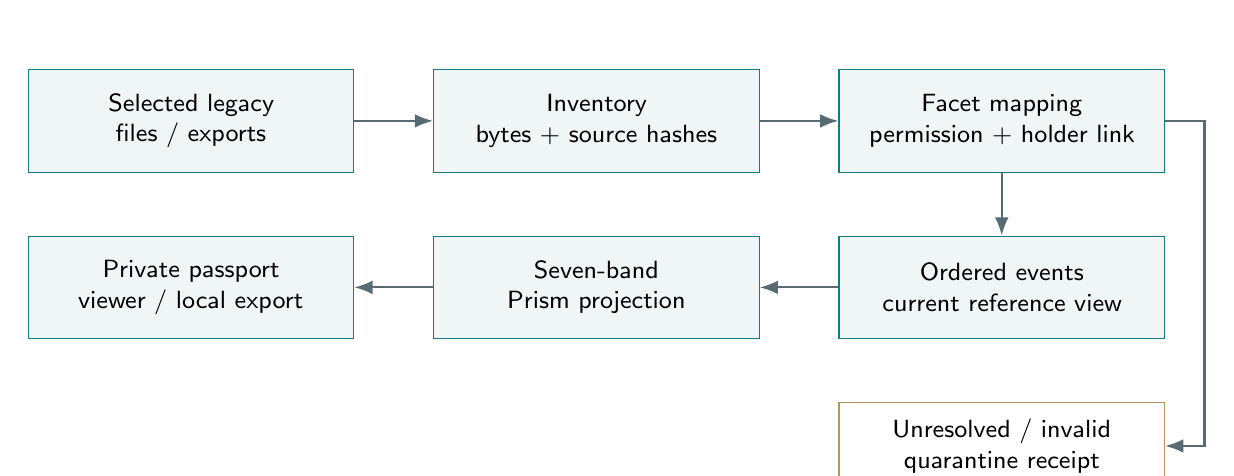
\begin{tikzpicture}[>=Latex,node distance=8mm and 10mm,
 n/.style={draw=teal,fill=pale,align=center,font=\sffamily\small,minimum height=13mm,text width=39mm},
 a/.style={->,draw=slate,line width=.8pt}]
\node[n] (files) {Selected legacy\\files / exports};
\node[n,right=of files] (inv) {Inventory\\bytes + source hashes};
\node[n,right=of inv] (gate) {Facet mapping\\permission + holder link};
\node[n,below=of gate] (ledger) {Ordered events\\current reference view};
\node[n,left=of ledger] (spectra) {Seven-band\\Prism projection};
\node[n,left=of spectra] (display) {Private passport\\viewer / local export};
\draw[a] (files)--(inv);\draw[a] (inv)--(gate);\draw[a] (gate)--(ledger);
\draw[a] (ledger)--(spectra);\draw[a] (spectra)--(display);
\node[draw=gold,align=center,font=\sffamily\small,text width=39mm,minimum height=11mm,below=of ledger] (quar) {Unresolved / invalid\\quarantine receipt};
\draw[a] (gate.east) -- ++(.5,0) |- (quar.east);
\end{tikzpicture}
\caption{The implemented path is a local, one-holder metadata flow. Payload files remain in their original locations.}
\end{figure}

\subsubsection{Fixed semantics and variable records}
The facet registry, schema and operator versions form the fixed descriptive layer. Payload references and event records form the variable layer. The reference graph may connect many records to one object without merging their meanings. An event that corrects a record names its predecessor; it is not an in-place rewrite of the old event body.

\subsubsection{Admission is explicit}
The prototype admits only the source classes \texttt{synthetic}, \texttt{holder\_export}, \texttt{holder\_measurement} and \texttt{holder\_declaration}. Admission requires \texttt{permission=granted} and \texttt{link\_status=holder\_confirmed}. These are local assertions checked for consistency. Production authentication and the independent validity of a permission receipt are separate obligations.

A mismatched holder, unsupported inferred attribute, withheld permission, unknown facet, conflicting record version or inconsistent digest/length pair is quarantined. The receipt records a reason and a sequence number, not the rejected record's potentially sensitive body.

\subsubsection{Storage and disclosure are separate}
The prototype writes ordinary local JSON. It does not encrypt files or implement an access-control server. A production passport needs secure storage, authenticated holder sessions, per-purpose disclosure and recovery procedures before real sensitive records are used. The visible spectrum is a private view; it is not an automatically published global identifier.

Withdrawal stops the current projection of a link. It is not a promise that original source files, backups or previously received copies have been erased. Deletion and retention require their own storage actions and receipts.

\newpagehead{The legacy migration workflow}
\subsubsection{1. Choose a finite source scope}
Select a folder of your own exports or records you are authorized to manage. Keep originals in place. Write down what the batch should contain, what is intentionally excluded, and which other people occur in shared records. Do not guess access to data claimed to be held by an intelligence service.

\subsubsection{2. Inventory before interpretation}
Run the local indexer. It reads bytes to calculate size and SHA-256, skips symlinks, checks for changes during a read, and enforces a default 100 MiB per-file budget. It does not upload, copy payloads, OCR documents or classify content.
\begin{lstlisting}
python tools/inventory.py --root /path/to/my_exports \
  --out /path/to/private_inventory.json
\end{lstlisting}
The inventory contains relative filenames, so treat it as private. File modification time is not silently substituted for the time of the experience described by a file.

\subsubsection{3. Assign facets manually}
In chosen inventory rows, replace \texttt{facet\_id: null} with a registered ID such as \texttt{F26} for authored work. Leave unknown rows unassigned. This step classifies record type; it does not infer the person's beliefs, desires, health or relationships from file content.

\subsubsection{4. Confirm authority and subject links}
Use a private opaque holder reference. Both confirmations are required by the importer:
\begin{lstlisting}
python tools/migrate.py --inventory /path/to/private_inventory.json \
  --holder holder:my-private-alias --out /path/to/my_prism \
  --confirm-authorized --confirm-holder-links
\end{lstlisting}
The importer writes \texttt{passport.json}, \texttt{snapshot.json} and a migration receipt. Unassigned rows are counted as unmapped; rejected rows are counted as quarantined. Observation times remain unknown unless a later explicit record supplies them.

\subsubsection{5. Reconcile and inspect}
Open \texttt{app/index.html}, then choose your local \texttt{snapshot.json}. Compare the counts with the source inventory. Check stale data, unknown timestamps, duplicate content and uncertain source links. Corrections and withdrawals use explicit event operations, not hidden replacement of the evidence.

\subsubsection{6. Export, preserve and stop}
Save the verified metadata snapshot and its receipt with the original files or a separately managed secure copy. Test restoration. Record what remains unmapped and the next concrete migration task, then end the session. This is an \textbf{index-and-link migration}; the tool does not move or back up the original payloads. A full storage migration adds a byte-copy and restore-verification stage.

\newpagehead{Sensory measurements and semantic restraint}
\subsubsection{Gaze is a measurement channel, not a private-trait label}
A gaze stream may contain positions, device coordinates, fixation durations, calibration and uncertainty. An iris template is a different kind of biometric record. Neither the UU ID minimum nor the log-polar address map supplies a decoder for sexual orientation, religious belief, intention, honesty or mental state. The source dialogue asserts such a connection but supplies no labelled measurement model or validation dataset. \source{S5; B, Sections 7 and 9}

\begin{center}\small\begin{tabularx}{\textwidth}{@{}p{.29\textwidth}Xp{.27\textwidth}@{}}\toprule
\textbf{Source observation} & \textbf{Permitted record description} & \textbf{Not a derived output here}\\\midrule
Gaze point and duration & An authorized fixation observation with coordinates and time. & Sexuality, belief or hidden desire.\\[7pt]
A displayed rainbow symbol & A visual item in its recorded context, when authorized. & Participation, ideology or consent to monitoring.\\[7pt]
Listening or reading history & A holder-selected sequence of media records. & A definitive personal belief or identity class.\\[7pt]
Physiological reading & The recorded quantity, unit, method and uncertainty. & A medical diagnosis or a moral score.\\[7pt]
Voluntary declaration & A statement supplied by the holder, with its provenance. & An immutable fact inferred from unrelated data.\\\bottomrule
\end{tabularx}\end{center}

\subsubsection{Unknown remains a first-class result}
An absent sensor, unavailable export, unknown event time or unresolved account link stays explicitly unknown. The system does not encode unknown as an observed zero. Missing location is not the coordinate $(0,0)$; an absent response is not a negative belief; a zero UU threshold deviation is not proof of complete knowledge.

\subsubsection{Multiple people require multiple permissions}
An individual's archive can contain other people's speech, faces, messages and contact details. Holder ownership of a device does not automatically settle every participant's permission. The proposed production adapter records participant scope, minimizes incidental information and avoids publishing contact graphs or raw shared recordings through the passport view. This edition includes no population-search or cross-holder aggregation routine.

\begin{note}{The user-controlled scope of this release}
The color vocabulary can cover records from many parts of life without claiming to observe every part of life. The practical unit is a labelled, authorized record with a stated origin, not a hidden category assigned to a person.
\end{note}

\newpagehead{The rainbow passport in use}
\begin{figure}[H]\centering

\includegraphics[width=\textwidth,height=.71\textheight,keepaspectratio]{figures/prism_viewer.png}
\caption{The shipped offline viewer, populated by synthetic metadata. The band names and facet IDs are stable; counts and source-time statuses change with the selected snapshot.}
\end{figure}

The top row shows active record links, distinct referenced objects, referenced bytes and withdrawn links. Each rainbow band shows which of its five facets has admitted data and which declared import targets are met. The detailed table below the screenshot carries all 35 facet IDs and their individual status and timestamps.

The \emph{Hide private details} control conceals holder references, counts, source times and digests in the displayed view. It is a presentation toggle, not encryption or a separate permission boundary. The underlying local tab still holds the loaded snapshot. Export is disabled while that concealed view is selected.

\newpagehead{Record format, snapshots and credential boundaries}
An admitted record has an ID, a holder reference, a facet ID, source metadata, a permission declaration, subject-link status, source and receipt times, a payload digest, a byte size and an assertion kind. A correction additionally names \texttt{supersedes}, the digest of the previous record version.

\begin{lstlisting}
{
  "record_id": "demo:F26",
  "holder_ref": "holder:synthetic-001",
  "facet_id": "F26",
  "source_ref": "synthetic:authored-work",
  "source_kind": "synthetic",
  "permission": "granted",
  "link_status": "holder_confirmed",
  "observed_at": null,
  "received_at": "2026-09-11T11:59:00Z",
  "payload_sha256": "<64 lowercase hexadecimal characters>",
  "byte_size": 48,
  "assertion_kind": "synthetic"
}
\end{lstlisting}
The digest placeholder above is explanatory; \texttt{verification/demo/input\_records.json} contains actual valid example digests. Raw sensory values and private documents are not placed in this public example.

\subsubsection{Canonical snapshot and ordered event record}
An event contains sequence, kind, predecessor hash and body. Its hash is calculated over those fields. A snapshot records the registry hash, plan, complete labelled facet view, counts, last event hash and its own canonical digest. Canonicalization is the edition's UTF-8 JSON rule: sorted object keys, preserved array order, compact separators and finite numbers.

Restoration replays the event bodies and compares the reconstructed view with the saved snapshot. A digest helps detect inconsistency relative to the expected reference. An attacker who can replace both the content and the expected root can construct a different internally consistent archive. Hash chaining is not identity authentication, encryption or a digital signature.

\subsubsection{A passport view is not automatically an issued credential}
W3C's credential model separates issuer, holder and verifier. It also distinguishes verifying an authentic, current statement from establishing the truth of every claim. The new JSON format is a local Prism construction; it does not claim W3C credential conformance or governmental issuance. \source{E2, Sections 1.1--1.2}

A later credential integration would specify issuer trust, signing keys, expiry, revocation and the particular attributes a verifier needs. W3C's data-minimization guidance supports requesting only those attributes rather than disclosing the holder's whole archive. The current packet explicitly carries \texttt{credential\_status: not\_issued}. \source{E2, Section 8.9}

\newpagehead{Mass aggregation and divide et impera as a threat model}
The request's \emph{divide et impera} phrase expresses a concern that individually revealing streams could be used to partition and govern people. S5 develops that scenario through uniform symbols, packed words, inferred preferences and global groups. This version documents that scenario rather than converting it into a surveillance operator.

\subsubsection{Two different aggregation problems}
\textbf{Within-holder aggregation} reconciles one person's selected records and restores their ability to inspect, correct and selectively use them. This is the implemented problem.

\textbf{Cross-population aggregation} joins many people's records and can expose individuals through linkable identifiers or rare combinations. A multi-holder deployment is not a mere increase in the cell count of Gambit: it adds authorization boundaries, subject-resolution errors, inference risks and data-sharing decisions. This release does not implement a central population registry, sensitive-trait clustering or behavioral intervention engine.

\begin{center}\small\begin{tabularx}{\textwidth}{@{}p{.29\textwidth}X@{}}\toprule
\textbf{Risk in the scenario} & \textbf{Design response in the holder-governed branch}\\\midrule
A single public passport key links all activity & Use private holder references; separate context-specific identifiers in a production design.\\[7pt]
Colored groups become social rankings & Colors label record domains only; there is no individual rank, norm, threat score or target class.\\[7pt]
Unknown is converted into suspicion & Preserve missing, unmapped, withheld and unknown-time states without imputing traits.\\[7pt]
Metadata becomes compulsory full disclosure & A production verifier requests a purpose-specific presentation, not the complete sensor history.\\[7pt]
An incorrect account merge propagates & Require explicit holder links; quarantine uncertainty; retain corrections and predecessor versions.\\[7pt]
A dashboard becomes another engagement feed & Use finite inventory and reconciliation sessions; no autoplay feed, recommendation ranking or persuasive notifications.\\\bottomrule
\end{tabularx}\end{center}

\subsubsection{Scaling without classifying people}
The extensible architecture can place independent holder stores behind the same public facet schema. Sharing a schema does not require sharing a global identity index. Any later statistical release needs its own purpose, contributor permission, disclosure analysis and independently specified aggregation mechanism. Even a small group count or an ostensibly anonymous spectrum can reveal information when combined with other records; this edition makes no anonymity guarantee.

W3C explicitly discusses identifier-based correlation and the risks of aggregating credentials. Those are relevant design concerns for a personal passport, independently of the source dialogue's intelligence scenario. \source{E2, Sections 8.4 and 8.13}

\newpagehead{What the source equations establish—and what they do not}
This page records the important mathematical distinctions in the supplied dialogue. The complete 15-entry concordance is in \texttt{spec/source\_concordance.json} and its CSV companion. This record is explicit so that the formalization does not silently substitute a different meaning for a source assertion.

\begin{center}\small\begin{tabularx}{\textwidth}{@{}p{.31\textwidth}X@{}}\toprule
\textbf{Dialogue formulation} & \textbf{Exact treatment in the sub-addendum}\\\midrule
Active-bit extraction is data harvesting & It is a transformation of an already supplied integer. Acquisition requires an independently specified source.\\[7pt]
A packed word represents a whole society & C8 packs supplied Boolean fields. A person's identity and behavior are not defined by that packing rule.\\[7pt]
Parity exposes every hidden deviation & Even-weight changes can preserve parity. The parity bit neither identifies the changed cell nor authenticates a sender.\\[7pt]
Hysteresis preserves every event forever & A latch retains bounded state, not an entire ordered trajectory. $0\to0\to0$ and $0\to1\to0$ have equal endpoints and equal event XOR.\\[7pt]
C15 guarantees every bit change spreads & C15 demonstrates one specified intervention, not universal sensitivity of all signals or people.\\[7pt]
A hash creates immutable human identity & A hash is a content reference. It is not an authorization, a proof of personhood or evidence that a record is true.\\[7pt]
A finite word contains all life history & The parent encoder is injective on its admitted finite state domain. Arbitrary additional history requires additional storage.\\[7pt]
Equal Hamming weights imply identical behavior & Different words can have the same weight. The Dutch 0--99 atlas supplies no human grouping theorem.\\[7pt]
The SDF makes an apparent social group real & C13 and the unsigned wrapper encode supplied state geometrically. They do not establish the origin or nature of a social group.\\[7pt]
Gaze or rainbow symbols expose private traits & Neither a labelled dataset nor a valid inference map is supplied. No such classifier is added.\\\bottomrule
\end{tabularx}\end{center}

\textbf{Retained result.} The corpus supplies typed definitions, explicit dependency structure, exact admitted-state encodings, staged updates and traceable representations. The Prism uses those mechanisms to make records inspectable. It does not turn a metaphor or a projection into evidence of universal surveillance. \source{B, Sections 2, 5, 7--9; S5}

\newpagehead{Executed example and verification record}
The demonstration is \texttt{synthetic-single-holder-16}. Its input contains 16 synthetic metadata links spanning all seven bands. F01 and F02 intentionally reference the same byte object through different facet links. One exact retry is submitted, four invalid attempts are quarantined, one record is corrected and the gaze link is withdrawn.

\begin{center}\begin{tabularx}{\textwidth}{@{}Xr@{}}\toprule
\textbf{Recorded quantity} & \textbf{Result}\\\midrule
Rainbow bands / registered facets & 7 / 35\\
Initial admitted synthetic links & 16\\
Active links after correction and withdrawal & 15\\
Distinct active referenced objects & 14\\
Active referenced bytes & 667\\
Duplicate attempts / quarantined attempts & 1 / 4\\
Withdrawn links / ordered events & 1 / 18\\
Fresh / stale active facets & 10 / 3\\
Unknown-time / clock-conflict active facets & 1 / 1\\
UU ID migration minimum & $0/1$\\
Whole declared plan complete & False\\
Event-chain verification / restore comparison & Passed / Equal\\\bottomrule
\end{tabularx}\end{center}

The referenced bytes are synthetic text-fixture sizes, not audio, iris or physiological recordings. One imported source clock is deliberately ahead of the view time. The unknown-time and stale cases are likewise explicit fixture choices. The as-of time is \texttt{2026-09-11T12:00:00Z}.

\subsubsection{New and retained verification are separate}
The \textbf{66 new Python test methods} check minimum algebra, source admission, holder isolation, consent flags, explicit self-report rules, duplicate handling, correction predecessors, unknowns, freshness, clock conflict, content-size consistency, event integrity, restore replay and the local inventory's file handling.

The retained V2 archive was independently unpacked and rechecked for this release. Its \textbf{126 tests}, \textbf{34 sealed definitions}, schema validation and direct/unsigned-field replay passed. These are the unchanged parent checks; they are not rebranded as human sensory validation.

The HTML viewer was exercised in Chromium: all 35 facet rows rendered; local JSON import, privacy concealment and replay controls passed; the checked interactions produced no JavaScript errors and no HTTP(S) requests. The test loaded the same HTML content in the browser harness; this environment's policy prevented direct \texttt{file:} navigation. No live sensor or agency integration was tested or implemented.

\begin{note}{Verification scope}
These results establish the recorded behavior of the included synthetic and file-metadata constructions. Performance at global scale, real sensor accuracy, secure multi-user access and official credential issuance are separate implementation projects.
\end{note}

\newpagehead{Archive contents and reproduction}
\begin{center}\small\begin{tabularx}{\textwidth}{@{}p{.26\textwidth}X@{}}\toprule
\textbf{Path} & \textbf{Contents}\\\midrule
\texttt{report/} & Revised integrated PDF, this sub-addendum, editable LaTeX and the calculated viewer image.\\[5pt]
\texttt{app/index.html} & Self-contained offline viewer with 18 synthetic replay frames and local snapshot import.\\[5pt]
\texttt{src/uu\_prism/} & Deterministic, holder-scoped metadata admission, snapshots, exact rational UU ID and replay.\\[5pt]
\texttt{tools/} & Inventory, migration, demo, viewer generation and verification scripts.\\[5pt]
\texttt{spec/} & Seven-band/35-facet catalogue, record and snapshot schemas, source concordance.\\[5pt]
\texttt{verification/} & Synthetic inputs and results, passport export, new test log, baseline test log and browser checks.\\[5pt]
\texttt{baseline/} & The supplied V2.1 PDF and original V2 executable ZIP, preserved unchanged.\\[5pt]
\texttt{sources/} & Source titles, roles, exact local hashes and checked external references.\\[5pt]
\texttt{checksums/} & The file-by-file SHA-256 release manifest.\\\bottomrule
\end{tabularx}\end{center}

\subsubsection{Run the included example}
The core tools use Python 3.10 or later and the standard library. From the extracted project root:
\begin{lstlisting}
python tools/demo.py --out demo_run
python tools/verify.py
\end{lstlisting}
The verifier checks the release manifest, runs the new tests, repeats the synthetic example in a temporary directory and compares it to the recorded outputs. It also verifies that the saved passport restores to the same snapshot. It leaves the comparison targets unchanged.

\subsubsection{Additional verification}
\begin{lstlisting}
python tools/verify.py --schema --baseline
\end{lstlisting}
\texttt{--schema} uses the optional \texttt{jsonschema} package. \texttt{--baseline} unpacks the preserved V2 archive in a temporary directory and invokes its verifier. Its additional schema checks require the same optional dependency. The program reports missing dependencies or failed checks, rather than counting them as success.

\subsubsection{Rebuild the document}
The addendum is editable LaTeX. PDF assembly uses the included script and the preserved parent PDF. Figure reproduction can use the HTML viewer; the recorded image is already supplied. The prototype performs no automated install, network retrieval, covert capture or permission bypass.

\newpagehead{Sources and the scope of their use}
\subsubsection{B. Parent corpus}
\emph{Tom Klootwijk --- Unified Field Theory V2.1}, supplied 48-page PDF. The parent defines the UU ID calculus, tagged horizons, chronotemporal integral and historical minimum, fixed engine, state encodings, U4, UF2, C1--C16 and the monotheistic source--boundary addendum. Parent references in this appendix identify its section numbers or physical PDF pages. The unchanged file is included in \texttt{baseline/}.

\subsubsection{S5. New supplied dialogue}
\emph{Pasted markdown.md}, supplied with this request. Used for the sequence of prism, rainbow, signal separation, symbols, personal identity, total-harvesting and digital-passport concepts. Conversational interface fragments are omitted from the formal text. Its source assertions and the new design decisions are separately recorded in the 15-point concordance. The file's exact digest is retained; the raw dialogue is not duplicated in the software archive.

\subsubsection{E1. Historical PRISM terminology}
Privacy and Civil Liberties Oversight Board, \href{https://documents.pclob.gov/prod/Documents/OversightReport/054417e4-9d20-427a-9850-862a6f29ac42/2023\%20PCLOB\%20702\%20Report\%20(002).pdf}{\emph{Report on the Surveillance Program Operated Pursuant to Section 702}} (2023), printed pp. 3--4, physical PDF pp. 9--10. Used only for the provider/downstream versus backbone/upstream distinction in I.2. Consulted 11 September 2026. It is not used as proof of total collection or as current legal advice.

\subsubsection{E2. Digital credential roles and privacy}
W3C, \href{https://www.w3.org/TR/2025/REC-vc-data-model-2.0-20250515/}{\emph{Verifiable Credentials Data Model v2.0}}, Recommendation dated 15 May 2025. Relevant sections: 1.1--1.2 for roles and verification, 8.4 for identifier correlation, 8.9 for minimization and 8.13 for aggregation. Consulted 11 September 2026. This addendum adopts related design considerations but does not declare the prototype a conforming credential implementation.

\subsubsection{E3. Conventional UUID identifiers}
IETF, \href{https://www.rfc-editor.org/rfc/rfc9562.html}{\emph{RFC 9562: Universally Unique IDentifiers (UUIDs)}} (2024), Sections 4, 5.4 and 8. Used to distinguish a conventional identifier from the corpus's UU ID operator and from access authorization. Consulted 11 September 2026.

\subsubsection{E4. Accessible color semantics}
W3C Web Accessibility Initiative, \href{https://www.w3.org/WAI/WCAG22/Understanding/use-of-color.html}{\emph{Understanding Success Criterion 1.4.1: Use of Color}}. Used for the redundant text/ID labeling of the rainbow bands. Consulted 11 September 2026. Full accessibility conformance requires a separate evaluation beyond this single criterion.

\begin{note}{Source hierarchy}
The parent PDF supplies the retained mathematics. S5 supplies the user's conceptual scenario. E1--E4 supply the narrowly identified external context. The facet taxonomy, passport state, admission rules, interface, migration procedure and new propositions are explicitly \textbf{V2.1.1 constructions}.
\end{note}

\newpagehead{Subversion identity and incorporation record}
\textbf{Title:} Tom Klootwijk --- Unified Field Theory V2.1.1: UU ID Prism.\\
\textbf{Parent:} V2.1, interpreted as semantic version \texttt{2.1.0}.\\
\textbf{New component:} Appendix I, Rainbow Facets and the Personal Data Passport.\\
\textbf{Author:} Tom Klootwijk; NL200678942; 10-07-1990.\\
\textbf{Profile:} \texttt{UU-PRISM-35-1}.\\
\textbf{Implementation:} local, single-holder, metadata-only; synthetic demonstration.

\begin{center}\small\begin{tabularx}{\textwidth}{@{}p{.34\textwidth}X@{}}\toprule
\textbf{Requested element} & \textbf{Incorporation}\\\midrule
UU ID prism & Label-preserving facet projection and the source minimum operator, with a complete component vector.\\[7pt]
Rainbow spectra for all facets & Seven categorical bands and 35 extensible facet definitions. No unobserved trait is fabricated.\\[7pt]
Real-time digital passport & Timestamped view semantics, explicit freshness states, offline replay, local import and snapshot export.\\[7pt]
Mass NSA/PRISM aggregation & Source scenario documented; historical PRISM terminology separately checked; no agency link or covert collector.\\[7pt]
Divide et impera & Explicit governance threat model, separated from the holder-governed implementation.\\[7pt]
Migration instead of doomscrolling & Finite inventory, mapping, reconciliation, export and stop workflow.\\[7pt]
PDF and accompanying ZIP & Integrated volume, editable addendum, schemas, source, viewer, synthetic records, tests and manifest.\\\bottomrule
\end{tabularx}\end{center}

\subsubsection{Parent preservation}
The integrated volume replaces the cover and appends this appendix after the original 48-page parent sequence. Parent body pages 2--48 are preserved; their original edition markings, contents page and historical verification statements remain part of that baseline. The merged PDF's bookmarks add this appendix and its subsections. The new appendix starts on \textbf{physical PDF page 49}, continuing the printed page sequence at 46.

The original parent PDF and V2 ZIP remain unchanged in the new package. Their file hashes and the new release manifest distinguish those inherited artifacts from the added code and report. No parent operator record, canonical engine width, numerical transition, UU ID formula or monotheistic declaration is silently rewritten.

\begin{formal}{Canonical reading of the Prism}
The UU ID Prism makes the holder's admitted records visible as named, time-stamped facets. The rainbow is a shared legend, not a secret classifier or proof of what has been collected. The passport is a usable, revisable view of an explicit archive scope. Its value is inspectable provenance and controlled migration, not a promise to encode or govern the entirety of a human being.
\end{formal}
\end{document}
